\documentclass[a4paper,ngerman]{scrartcl}

\usepackage{amsmath}
\usepackage{amsfonts}
\usepackage{amssymb}
\usepackage[utf8]{inputenc}
\usepackage{graphicx}
\usepackage[ngerman]{babel}
\usepackage{hyperref}
\usepackage{float}
\usepackage{caption}
\usepackage{subcaption}
\usepackage{multirow}  %for tables
\usepackage{icomma} % Handle german comma as decimal point in numbers
\usepackage{units,siunitx} % Write units with correct spacing
\usepackage{upgreek} % provide non-italic greek letters
\usepackage{url}


% Formatting of table & figure captions
\captionsetup{font={sf,footnotesize},labelfont=bf,textfont=sl,skip=6pt}
\setlength{\abovecaptionskip}{6pt}
\setlength{\belowcaptionskip}{0pt}

\title{Quantenradierer}
\date{\today}
\author{Michel Rausch, Michael Eliachevitch}

\begin{document}

\maketitle
\tableofcontents
\thispagestyle{empty} % remove page number from abstract page
\newpage
\setcounter{page}{1}

\section{Einleitung}
\label{sec:einleitung}
In dem Versuch zum Quantenradierer geht es darum, mithilfe eines Mach-Zehnder-Interferometers 
die Welleneigenschaften von Licht zu veranschaulichen und diese sowohl mit der klassischen Optik
als auch quantenmechanisch zu interpretieren. Es soll außerdem untersucht werden, wie die Wellenfunktion
kollabiert, wenn durch einen Messvorgang die Information weitergegeben wird, welchen Weg ein Teilchen genommen hat, und
wie der Kollaps aufgehoben wird, wenn man diese Information mit einem "`Quantenradierer"' wieder löscht.
Zudem soll der Umgang mit einem Laser und dessen Justierung geübt werden.


\section{Theoretische Überlegungen}
\label{sec:theorie}

\subsection{Interferenz von Wellen, klassisch und quantenmechanisch}
\label{sec:interferenz}

\paragraph{Klassische Betrachtung:}
\label{par:klass}
In der klassischen Elektrodynamik werden Lichtstrahlen als elektromagnetische Wellen beschrieben, also Wellen im elektromagnetischen Feld,
und sind Lösungen der Maxwellschen Gleichungen. Das elektrische Feld $\vec{E}$ einer ebenen elektromagnetischen Welle breitet sich gemäß der
Gleichung

\begin{equation}
\vec{E}(\vec{x},t) = \vec{E_0} e^{i(\vec{k}\vec{x}-\omega t)}
\end{equation}

aus, wobei die Exponentialfunktion aus Bequemlichkeitsgründen verwendet wird, die Welle aber
als reell angenommen wird. Die Richtung des elektrischen Feldvektors $\vec{E}$ gibt die Polarisation der Welle an.

Die Intensität der Welle ist gegeben über 

\begin{equation}
I(\vec{x},t) = |\vec{E}(\vec{x},t)|^2 = \vec{E}(\vec{x},t) \cdot \vec{E}^*(\vec{x},t).
\end{equation}

Da einzelne Photonen die Energie $E_\gamma = \hbar \omega$ haben, folgt die Photonendichte $\eta_{ph}(\vec{x},t)$:

\begin{equation}
  \eta_{ph}(\vec{x},t) = \frac{I(\vec{x},t)}{\hbar \omega} = \frac{|\vec{E}(\vec{x},t)|^2}{\hbar \omega}.
\end{equation}

Wenn sich zwei Wellen überlagern, ist die entstehende Welle die Superposition beider Teilwellen.
Wir nehmen nun an, dass sich die Wellen in z-Richtung ausbreiten.
Im Interferometer wird eine ebene Welle mit einem Strahlteiler in zwei Teilwellen geteilt, die dann mit einem Strahlteiler wieder
zusammengeführt werden. Dabei erfährt eine der Wellen eine Laufzeitdifferenz $\Delta z$, was bei der Superposition zu
einem Phasenunterschied $\Delta z k_z$ führt. Aus der Superposition von zwei Wellen mit einem solchen Phasenunterschied
folgt eine Photonendichte

\begin{equation}
  \eta_{ph}(\vec{x},t) = \frac{1}{2} \vec{E}_0 \left( e^{i k_z z} + e^{i k_z (z + \Delta z)} \right) e^{i\omega t},
\end{equation}

was quadratisch zu einer Intensität von 

\begin{equation}
\label{eqn:intensitaet}
  \begin{split}
    I(z,t) &= \frac{|\vec{E_0}|^2 }{4} \left(e^{i k_z z} + e^{i k_z (z + \Delta z)} \right) \left(e^{-i k_z z} + e^{-i k_z (z + \Delta z)} \right)\\
    &= \frac{|\vec{E_0}|^2}{2}(1+\cos(k_z\Delta z) )\\
  \end{split}
\end{equation}

und einer entsprechenden Photonendichte $\eta_{ph}(z,t) = \frac{I(z,t)}{\hbar \omega}$ führt. Der vom Phasenunterschied abhängige
Kosinusterm wird als Interferenzterm bezeichnet, da ohne die Interferenz die Intensität nach der Vereinigung konstant $\frac{|\vec{E_0}|^2}{2}$
wäre. Da am Mach-Zehnder-Interferomter der Phasenunterschied durch die Divergenz an einer Linse entsteht, also vom der Position des Durchgangs
durch die Linse abhängt, sieht man an einem Schirm hinter dem zweiten Strahlteiler konzentrische Ringe, die durch diesen Interferenzterm
entstehen. Diese Ringe sind nur durch die Welleneigenschaften von Licht erklärbar.

\paragraph{Quantenmechanische Betrachtung:}
In der Quantenmechanik betrachtet man Licht zwar als Teilchen, da die Energie und Information gequantelt in Form von Photenen
transportiert, aber schreibt ihnen auch Welleneigenschaften zu. Das liegt daran, dass quantenmechanische Teilchen keine definite
Position haben. Stattdessen werden sie durch eine komplexe Wellenfunktion $\Psi(\vec{x})$ beschrieben, die eine Lösung der
komplexen Schrödingergleichung 
\begin{equation}
  i \hbar \frac{\partial}{\partial t} \Psi(\vec{x},t) = H \Psi(\vec{x},t),
\end{equation}
ist.

Deren Betragsquadrat gibt für jeden Ort im Raum die Aufenthaltswahrscheinlichkeit des Teilchens an:
\begin{equation}
  \rho(\vec{x},t) = |\Psi(\vec{x},t)|^2 = \Psi(\vec{x},t) \cdot \Psi^*(\vec{x},t).
\end{equation}

Bei Photonen ist die Aufenthaltswahrscheinlichkeit proportional zu der Photonendichte $\eta_{ph}$ aus der klassischen Betrachtung von elektromagnetischen Wellen. Die Lösungen der Schrödingergleichung für freie Photonen sind wie in der Elektrodynamik ebene Wellen der Form

\begin{equation}
  \Psi(\vec{x},t) = \Psi_0 e^{i(\vec{k}\vec{x}-\omega t)}.
\end{equation}

Somit lassen sich dir konzentrischen Ringe am Schirm vom Interferometer quantenmechanisch völlig äquivalent zur Elektrodynamik erklären,
mit einem identischen Interferenzterm der durch den Phasenunterschied zustandekommt,
nur dass man statt elektromagnetische Wellen die Wellenfunktion verwendet. \\

Interessant ist, dass auch einzelne Photonen durch eine Wellenfunktion beschrieben werden und es daher auch zu Interferenzeffekton kommt,
wenn man einzelne Teilchen in ein Interferometer schickt.


\subsection{Kollaps der Wellenfunktion und die "`Welcher-Weg"'-Information}
\label{sec:welcher-weg}
Die quantenmechanische Interpretation der Entstehung von Interferenzmustern mithilfe der Überlagerung von Wellenfunktionen lässt sich auch
mithilfe von Pfadintegralen interpretieren. Dabei nimmt man an, dass jedes Photon von der Lichtquelle zum Punkt auf dem Schirm, wo es auftrift,
alle möglichen Wege "`gleichzeitig"' nimmt. Am Ende wird über alle möglichen Wege integriert, wobei jeder Weg mit seiner Wahrscheinlichkeit
gewichtet und mit der zugehörigen Phase versehen wird.\\

Wenn man nun bestimmt, welchen Weg ein Photon genommen hat, zum Beispiel indem man es mit einer Polarisation markiert, wie es in unserem Versuch gemacht wird, dann nimmt man dem Teilchen sozusagen die Möglichkeit, alle Wege zu nehmen, man "`zwingt"' es den Weg zu nehmen, der seiner 
Polarisation entspricht. Da ist selbst dann der Fall, wenn die Markierung passiert, nachdem das Teilchen den Spalt oder in unserem Fall den Strahlteiler passiert hat, es entscheidet sich sozusagen nachträglich für einen der Wege.\\

In dem man das Photon markiert, hat man einen Messvorgang durchgeführt. Im Wellenbild sagt man, dass die Wellenfunktion kollabiert, sie nimmt also einen ihrer Eigenzustände an, welcher einem der Wege entspricht. Dadurch verschwindet das Interferenzmuster. Wenn man die "`Markierung"' des Photons wieder entfernt, also die sogenannte "`Welcher-Weg"'-Information wieder löscht, kann das Photon wieder beide Wege nehmen und das Interferenzmuster taucht wieder auf. Genau das macht man bei einem sogenannten "`Quantenradierer"'.

\clearpage
\section{Das Mach-Zehnder-Interferometer und dessen Aufbau}
\label{sec:mach-zehnder}

\subsection{Aufbau eines einfachen Interferometers}
\label{ssec:interferomter-einfach}

Die theoretischen Überlegungen können in Interferometern geprüft werden. 
In einem einfachem Strahlteilungsinterferometer, wie in Abbildung \ref{fig: Interferometer-einfach} gezeigt. 
Eine planare Welle, hier Licht, wird mit einem halbtransparentem Spiegel in Wellen A und B aufgeteilt. Der Strahl A (rot im Bild) passiert den Strahlteiler und das Interferometer. 
Der zweite wird über Spiegel umgelenkt und erhält so eine längere Laufzeit, mit Gangunterschied $\Delta z$. 
Am zweiten Strahlteiler rekombinieren die Wellen. Dies wurde in \ref{sec:interferenz} beschrieben.

\begin{figure}
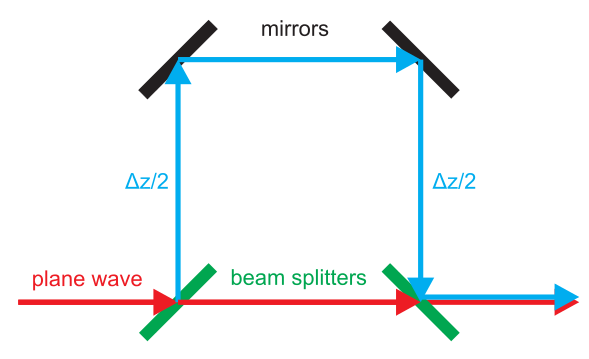
\includegraphics[width=0.7\textwidth]{interferomter-einfach.png}
\caption{Einfaches Interferometer, zur Strahlteilung und -rekombination, mit dem Laufzeitunterschied $\Delta z$ [\ref{ref:mappe}]}
\label{fig: Interferometer-einfach}
\end{figure}

\subsection{Quantenradierer}
\label{ssec:quantenradierer}

Man kann man die Eigenschaften von Photonen wie die Polarisation, und somit die Wellenfunktion, ändern. 
Bei anderen Quanten kann auch zum Beispiel der Spin manipuliert werden.

In diesen Versuch wird das Mach-Zehnder-Interferometer, wie in Abbildung \ref{fig:mach-zehnder}, verwendet. Dieses teilt eine eintreffende Welle auf. Die eintreffende Welle ist beschrieben durch ihr elektrisches Feld
 
\begin{equation}
\vec{E_0} = E_0 \ \begin{pmatrix} 1\\ 0 \end{pmatrix}
\end{equation}

Die Teilstrahlen A 	und B werden unterschiedlich polarisiert, mit Polarisationswinkeln von $45^{\circ}$ und $-45^{\circ}$. 
Hieraus ergeben sich

\begin{equation}
\vec{E_A} = \frac{E_0}{2 \sqrt{2}} \ \begin{pmatrix} 1\\ 1 \end{pmatrix} \ e^{i (k_z z -\omega t)}
\end{equation}
und
\begin{equation}
\vec{E_B} = \frac{E_0}{2 \sqrt{2}} \ \begin{pmatrix} 1\\ -1 \end{pmatrix} \ e^{i (k_z (z + \delta z) -\omega t)} .
\end{equation}

Hierbei wurde ohne Einschränkung der Allgemeinheit angenommen, dass sich die Wellen in z-Richtung ausbreiten. 
Der Gangunterschied $\Delta z$ stammt im Experiment von einer Linse, die eine kleine Divergenz der Strahlen verursacht.

\begin{figure}
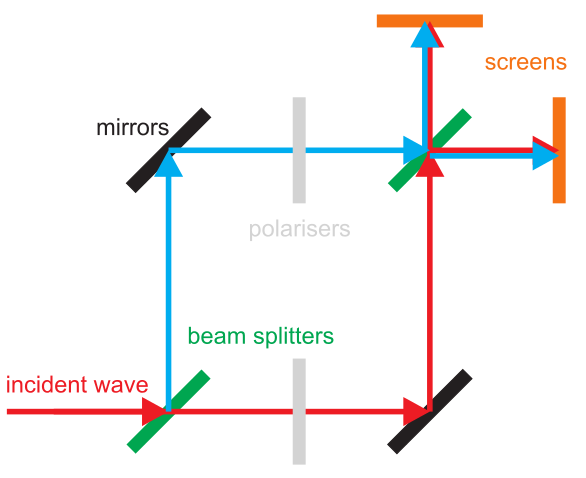
\includegraphics[width=0.7\textwidth]{mach-zehnder.png}
\caption{Skizze eines Mach-Zehnder-Interferomters mit Polarisatoren ($45^{\circ}$ und $-45^{\circ}$) [\ref{ref:mappe}]}
\label{fig:mach-zehnder}
\end{figure}

Durch die Wahl der Polarisation sind die Wellen A und B offensichtlich orthogonal. Der Interferenzterm aus Gleichung \ref{eqn:intensitaet} verschwindet. Es gilt somit der klassische Fall für die Intensität
\begin{equation}
I(z,t) = \frac{|\vec{E_0}|^2}{2}.
\end{equation}
Es ist somit kein Interferenzmuster sichtbar. 
Ohne Polarisationsfilter wäre ein ringförmiges Interferenzmuster zu erwarten.
Mit einem dritten Polarisator, der vor einem Abbildungsschirm montiert wird, kann man das Muster wieder sichtbar machen. 
Ist der Polarisator auf $0^{\circ}$ gestellt, ergeben sich die Teilwellen als

\begin{equation}
\vec{E_A} = \frac{E_0}{4} \ \begin{pmatrix} 1\\ 0 \end{pmatrix} \ e^{i (k_z z -\omega t)}
\end{equation}
und
\begin{equation}
\vec{E_A} = \frac{E_0}{4} \ \begin{pmatrix} 1\\ 0 \end{pmatrix} \ e^{i (k_z z -\omega t)}.
\end{equation}

Hier verschwindet der Interferenzterm offensichtlich nicht und das Muster wird wieder erkennbar. Gleichung \ref{eqn:intensitaet} bleibt somit

\begin{equation}
I(z,t) = \frac{|\vec{E_0}|^2}{2} \ (1+\cos(k_z\Delta z) ).
\end{equation}

Man sieht deutlich die Signifikanz der "'Welcher-Weg"'-Information aus \ref{sec:welcher-weg} und die Herkunft des Namens "'Quantenradierer"'.


\section{Versuchsdurchführung}
\label{sec:versuchsdurchfuhrung}

\subsection{Aufgabe 1: Aufbau}
\label{ssec:aufbau}

Der Aufbau des Arbeitsplatzes ist in Abbildung \ref{fig:aufbau} gezeigt. Der Strahlengang erfolgt wie in Abbildung \ref{fig:mach-zehnder}. Im folgenden erden folgende Beschreibungen verwendet:
\[
\begin{matrix}
\textbf{BS 1/2}	&	Stahlteiler 1/2 \\
\textbf{M 1/2}	&	Spiegel 1/2 \\
\textbf{Pol 1/2}	&	Polarisator 1/2 \\
\textbf{S 1/2}	&	Schirm 1/2 \\
\end{matrix}
\]

\begin{figure}
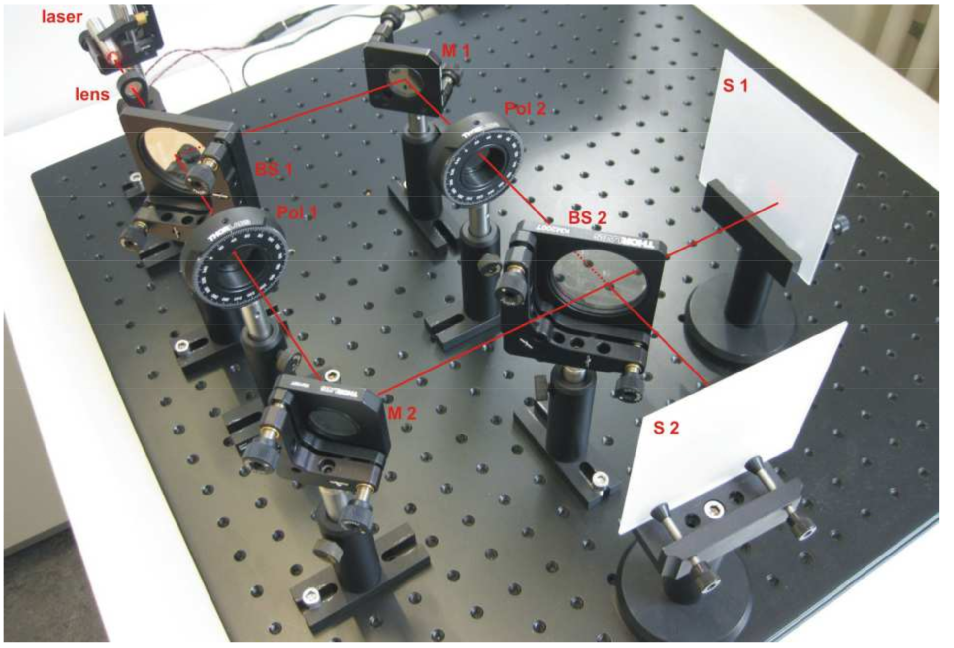
\includegraphics[width=\textwidth]{aufbau.png}
\caption{Aufbau des Arbeitsplatzes [\ref{ref:mappe}]}
\label{fig:aufbau}
\end{figure}


\paragraph{Ausrichtung des Lasers}
Der Laser wird an einer Ecke des stabilisiertem "'Kinematic VGroove"'-Steckbrettes montiert. 
Auf einem Papier wird die vertikale Position des Lasers markiert. 
Mit dem Papier wird die Position des Strahles auf gegenüberliegenden Seite verglichen und mit dessen Hilfe die vertikale Ausrichtung eingestellt.  

\paragraph{Linsenausrichtung}
Mit einem Schirm wird der Laser abgebildet. Die Linse wird in den Laser gehalten und so justiert, das die Position des Punktes der ohne Linse entspricht.

\paragraph{Ausrichtung des ersten Strahlteilers (BS1)}
Der Strahlteiler wird in den Pfad Lasers gestellt, sodass der Laser in die Mitte trifft. 
Der horizontale Winkel wird so justiert, das der reflektierte Strahl parallel zu dem Steckbrett ist. 
Die vertikale Einstellung erfolgt analog zur Linse.

\paragraph{Ausrichtung der Spiegel (M1/2)}
Die Spiegel werden wie in Abbildung \ref{fig:aufbau} montiert, sodass der Laser sie zentral trifft. 
Mithilfe des Abbildungsschirms werden sie justiert, das sich die Teilstrahlen an der künftigen Postion des zweiten Strahlteilers bündeln. 

\paragraph{Ausrichtung des zweiten Strahlteilers (BS2)}
Der Strahlteiler wird nun mit seinem Zentrum möglichst genau an die im letzten Schritt ermittelte Position montiert. Mit vertikalen Justierungen werden die heraustretenden Strahlen mit dem Steckbrett parallelisiert.

Die Abbildungsschirme werden positioniert. BS2 wird so eingestellt, das die Strahlen auf den Schirmen gespiegelt sind. Dies bedeutet, das, falls Strahl A auf S1 links unten zu B ist, muss B auf S2 im gleichen Maß links unten zu A sein.


\paragraph{Beam Walk anwenden}
Mit folgendem iterativem Verfahren werden die Feineinstellungen vorgenommen.
\subparagraph{1.}
Erster Spiegel wird eingestellt, sodass der Strahl den ersten erwünschten Punkte trifft
\subparagraph{2.}
Zweiter Spiegel wird eingestellt, sodass der Strahl den zweiten erwünschten Punkte trifft

Mit diesem Verfahren wird erst BS1 und M1 fein justiert. Strahlen B und A sollen sich an BS2 im Zentrum treffen.
Sollten auf S1 die Strahlen nicht aufeinander treffen, wird die Ausrichtung des zweiten Strahlteilers wiederholt.

Ist kein Ringmuster erkennbar, sonder lediglich ein Streifenmuster, sind die Strahlen nicht korrekt eingestellt. Bei horizontalen Streifen müssen M1 und M2 vertikal eingestellt werden und umgekehrt.

\subsection{Aufgabe 2}
Die Polarisatoren werden in den Strahlengang gebracht. Die Muster werden bei unterschiedlicher Polarisation, realisiert durch Drehen der Polarisatoren, beobachtet. Dies wird mit den Erkenntnissen aus Kapitel \ref{sec:welcher-weg} erklärt.

\subsection{Aufgabe 3}

Mit einem dritten Polarisator wird einer der beiden Strahl aus dem zweitem Strahlteiler (BS2) polarisiert und mit dem anderem Abbild verglichen. Es werden die Winkel $\pm 45^\circ$ gegenüber der anderen Polarisatoren verwendet. Die Erwartungen  sind in Kapitel \ref{ssec:quantenradierer} erläutert.

\subsection{Aufgabe 4}

In diesem Gedankenexperiment wird überlegt, was sich ändert, wenn der Laser durch eine Ein-Photonen-Quelle ersetzt wird. Über eine hohe Zeit gemittelt wäre es klassisch zu erwarten, dass sich kein Interferenzmuster bildet. Quantenmechanisch jedoch bleibt es erhalten.



\clearpage
\section{Quellen}
\begin{enumerate}
\item Vorbereitungsmappe \label{ref:mappe}
\end{enumerate}



\end{document}
